%& -job-name=test_name
%%%%%%%%%%% DOC CLASS & PACKAGES %%%%%%%%%%%%
\documentclass[11pt,letterpaper]{article}
\usepackage{graphicx,enumerate,amsmath,titlesec,amssymb,microtype,sectsty,float,subcaption}
\usepackage[bottom]{footmisc}
\usepackage[hidelinks]{hyperref}

%\usepackage[left=1.5cm,right=1.5cm,top=2cm,bottom=1cm]{geometry}
\usepackage[left=.75in,right=.75in,top=.75in,bottom=.75in]{geometry}


% Set Paragraph Spacing 
\setlength{\parskip}{0pt}
\setlength{\parindent}{0pt}

% Footnotes - Gap & Force to Bottom
\setlength{\footnotesep}{\baselineskip}
\usepackage[bottom]{footmisc}

%%%%%%%%%%% SECTION HEADING FONT %%%%%%%%%%%%
\usepackage[T1]{fontenc}
\sectionfont{\scshape}
\subsectionfont{\scshape}
\subsubsectionfont{\scshape}

% Bold right arrow
\newcommand{\baro}{\pmb{\rightarrow}}



\begin{document}



%%%%%%%%%%% TITLEPAGE %%%%%%%%%%%%%
\begin{center}
  \Huge{\textsc{\textbf{UCSB ECE Controls Lab TA Manual}}}
  \vspace{0.5cm}
  \\ \textbf{\textsc{By} \large{\textsc{Max Crisafulli}}}
  \vspace{0.2cm}
  \\ \textsc{September 2024}

  \vspace{\fill}

\begin{figure}[H]
    \centering
    \includegraphics[width=1\textwidth]{./Figures/IP02-Inverted-Pendulum_graphics.jpg}
    % \vspace{-1.75cm}
    % \caption*{Quanser Inverted Pendulum System}
\end{figure}

\vspace{\fill}


\textsc{This document lives at} \\
\url{https://github.com/MaxCrisafulli/UCSB-ControlsLab-Manual-2024}
\end{center}
\thispagestyle{empty}

%%%%%%%%%%% SKIPPED PAGE  %%%%%%%%%%%%%
\newpage
\phantom{}
\thispagestyle{empty}
\newpage
\setcounter{page}{1}

%\tableofcontents

\section{TA Manual for the UCSB ECE Controls Lab}
This document is to act as a guide for TAs in setting up the Quanser inverted pendulum cart hardware in the UCSB ECE Controls Lab (Harold Frank Hall 3120A). This guide is an update of the existing manual, located at:
\[ \text{ \url{https://github.com/justinpearson/UCSB-Quanser-Inverted-Pendulum-Lab-Manual}}\]
This updated guide will live (and hopefully be maintained) at 
\[\text{\url{https://github.com/MaxCrisafulli/UCSB-ControlsLab-Manual-2024}}\]
\subsection{Hardware In The Lab}
The ECE147ABC labs make use of the Quanser `Linear Servo Base Unit with Inverted Pendulum'. This manual will detail the setup of just the cart system, with motor voltage as input and linear position as output. There are 3 main components of the hardware setup, with each of which being explained below.

\subsubsection{Q4 DAQ Board}
The SIMULINK model that interfaces with the hardware interacts with the world via the Q4 HIL control card and DAQ (Data Acquisition Board). The control card is inside the lab PCs connected via PCIe and interfaces with the DAQ board via the two gray ribbon cables. Ensure that these are connected properly and that the red Status LED is lit, indicating that the board is powered.
\begin{figure}[H]
  \centering
  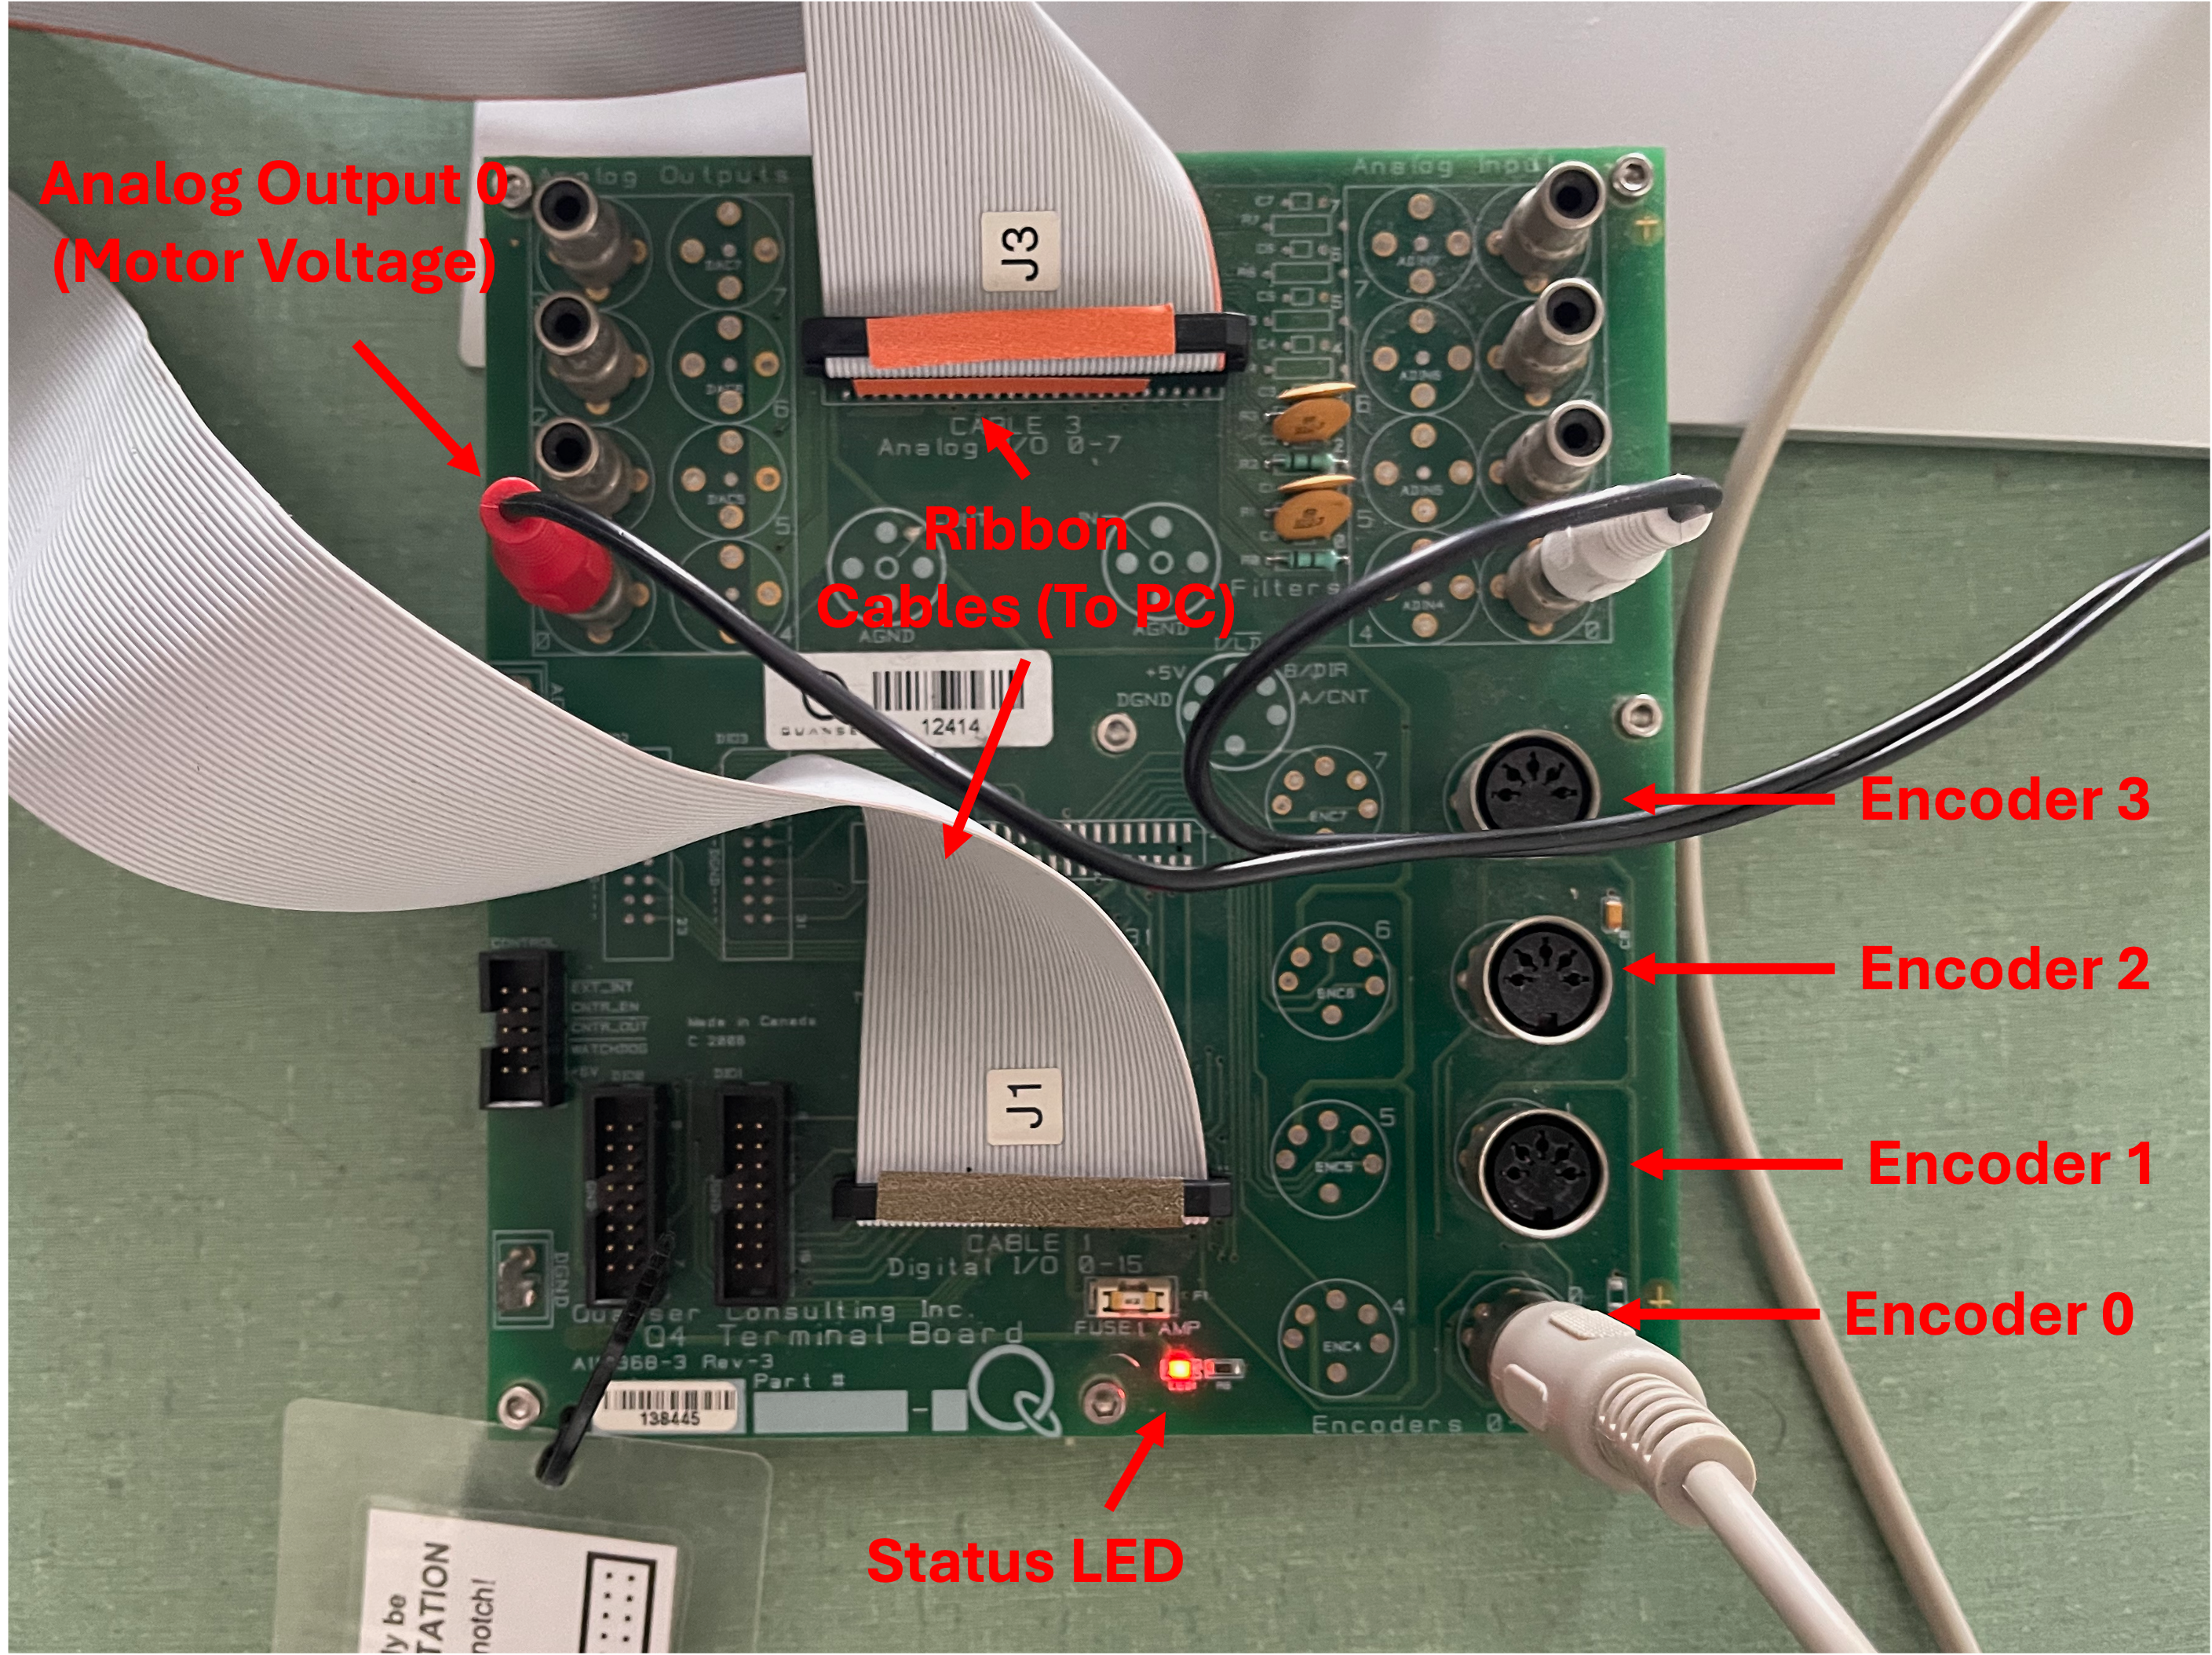
\includegraphics[width=.75\textwidth]{./Figures/DAQboard_annotated.png}
  \caption{Quanser Q4 Terminal DAQ Board}
\end{figure}
The DAQ board uses the four encoder ports to read signals from the hardware. Generally, Encoder 0 is used for the linear position encoder. In the top left corner of the board are the Analog Outputs, Analog Output 0 is used to drive the amplifier box which ultimately drives the cart motor.



\subsubsection{VoltPAQ-X1 Amplifier}
The Quanser VoltPAQ-X1 Amplifier is powered from a standard wall socket, and turned on via a switch at the back of the box. Make sure that the green status LED in the center of the amplifier diagram is lit, indicating that the amplifier is powered on. Also check that the Amplifier Gain switch is set to 1x.


\begin{figure}[H]
  \centering
  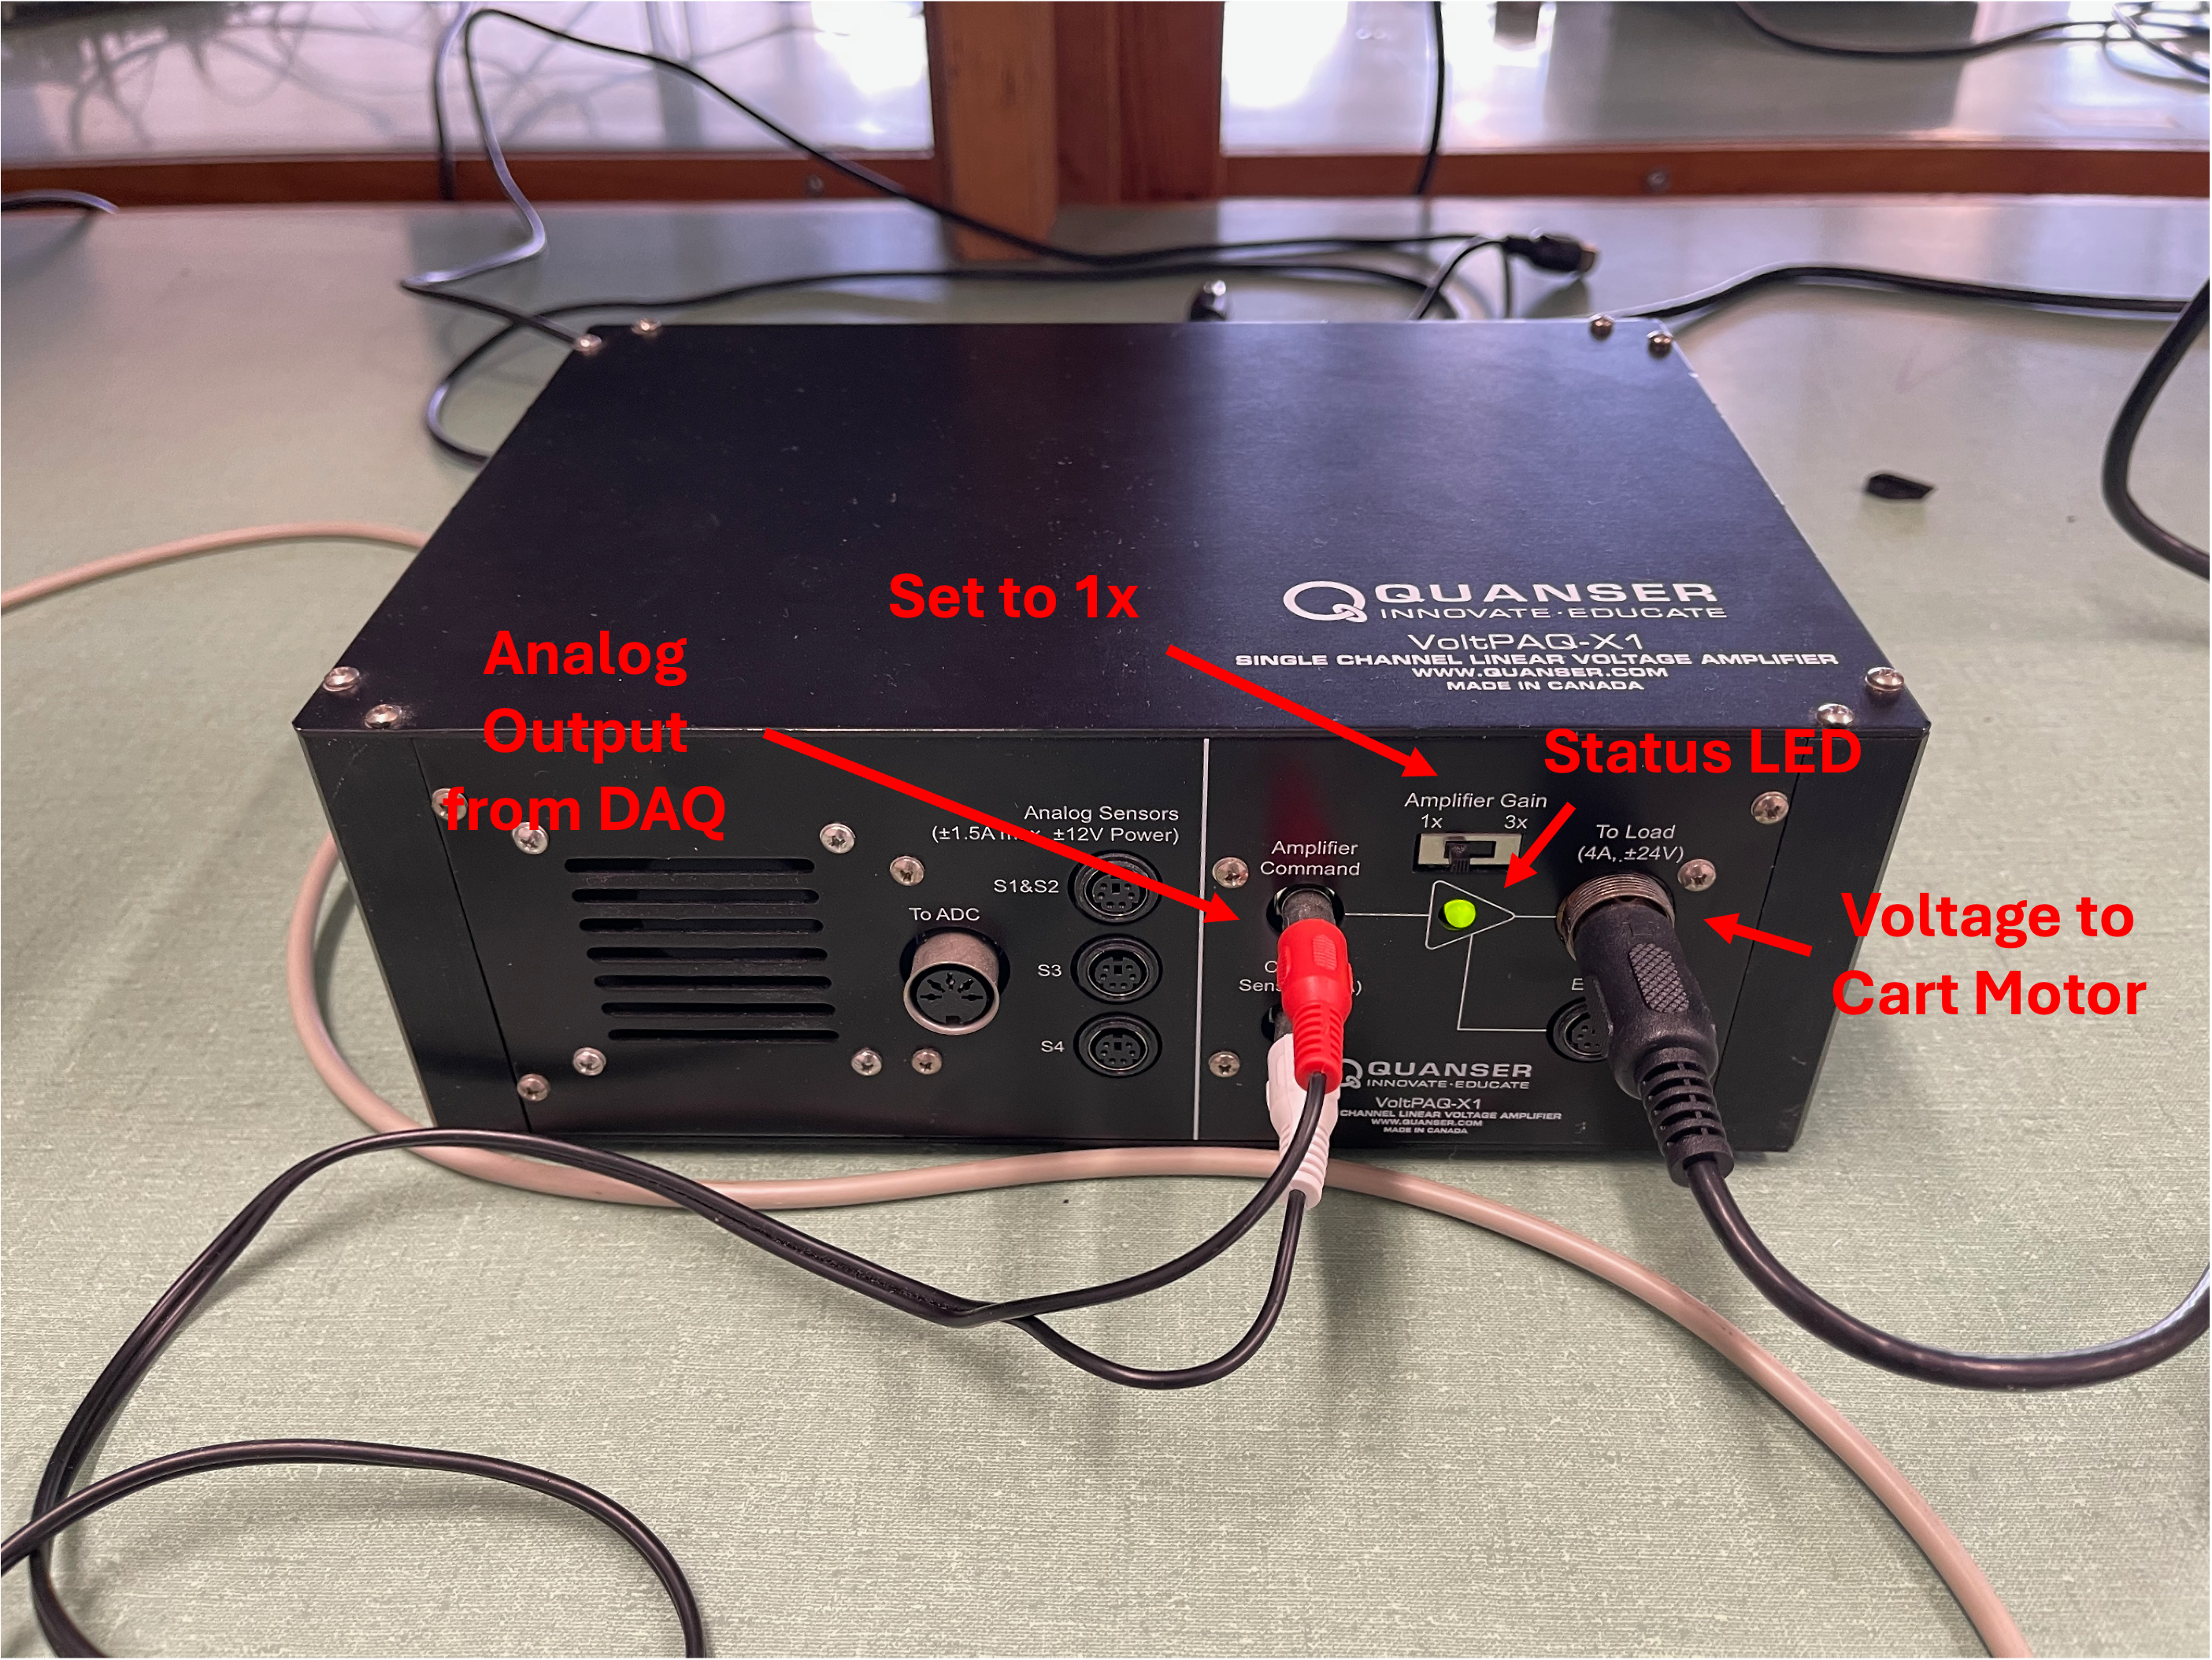
\includegraphics[width=.75\textwidth]{./Figures/amplifier_annotated.png}
  \caption{Quanser VoltPAQ-X1 Linear Voltage Amplifier}
\end{figure}

The red AV cable coming from Analog Output 0 on the DAQ board should be connected to the Amplifier Command (input) port. The white AV cable should be connected to Current Sense on the amplifier and Analog Input 0 on the DAQ board, although this is not necessary. \\

The output of the amplifier (To Load) is what drives the motor onboard the cart. Check that all the cable connections are correct and that the cable going to the motor has enough slack to allow the cart to move along the track. 

\subsubsection{Inverted Pendulum Cart System}
The cart system has 2 encoder outputs and 1 analog voltage input. The positions of these ports may vary between the carts but in general they are as depicted in Figure \ref{fig:cart}. You should check what each of the ports connect to before plugging anything in. \\

The cart controls its position along the track with the smaller motor drive wheel, which is driven by the motor voltage coming from the amplifier. The larger position encoder wheel measures the relative position along the track from the time that the program was initialized in `ticks'. The conversion ratio from ticks to inches is approximately 5000 ticks per 6 inches or 35000 ticks per 1m.
\begin{figure}[H]
  \centering
  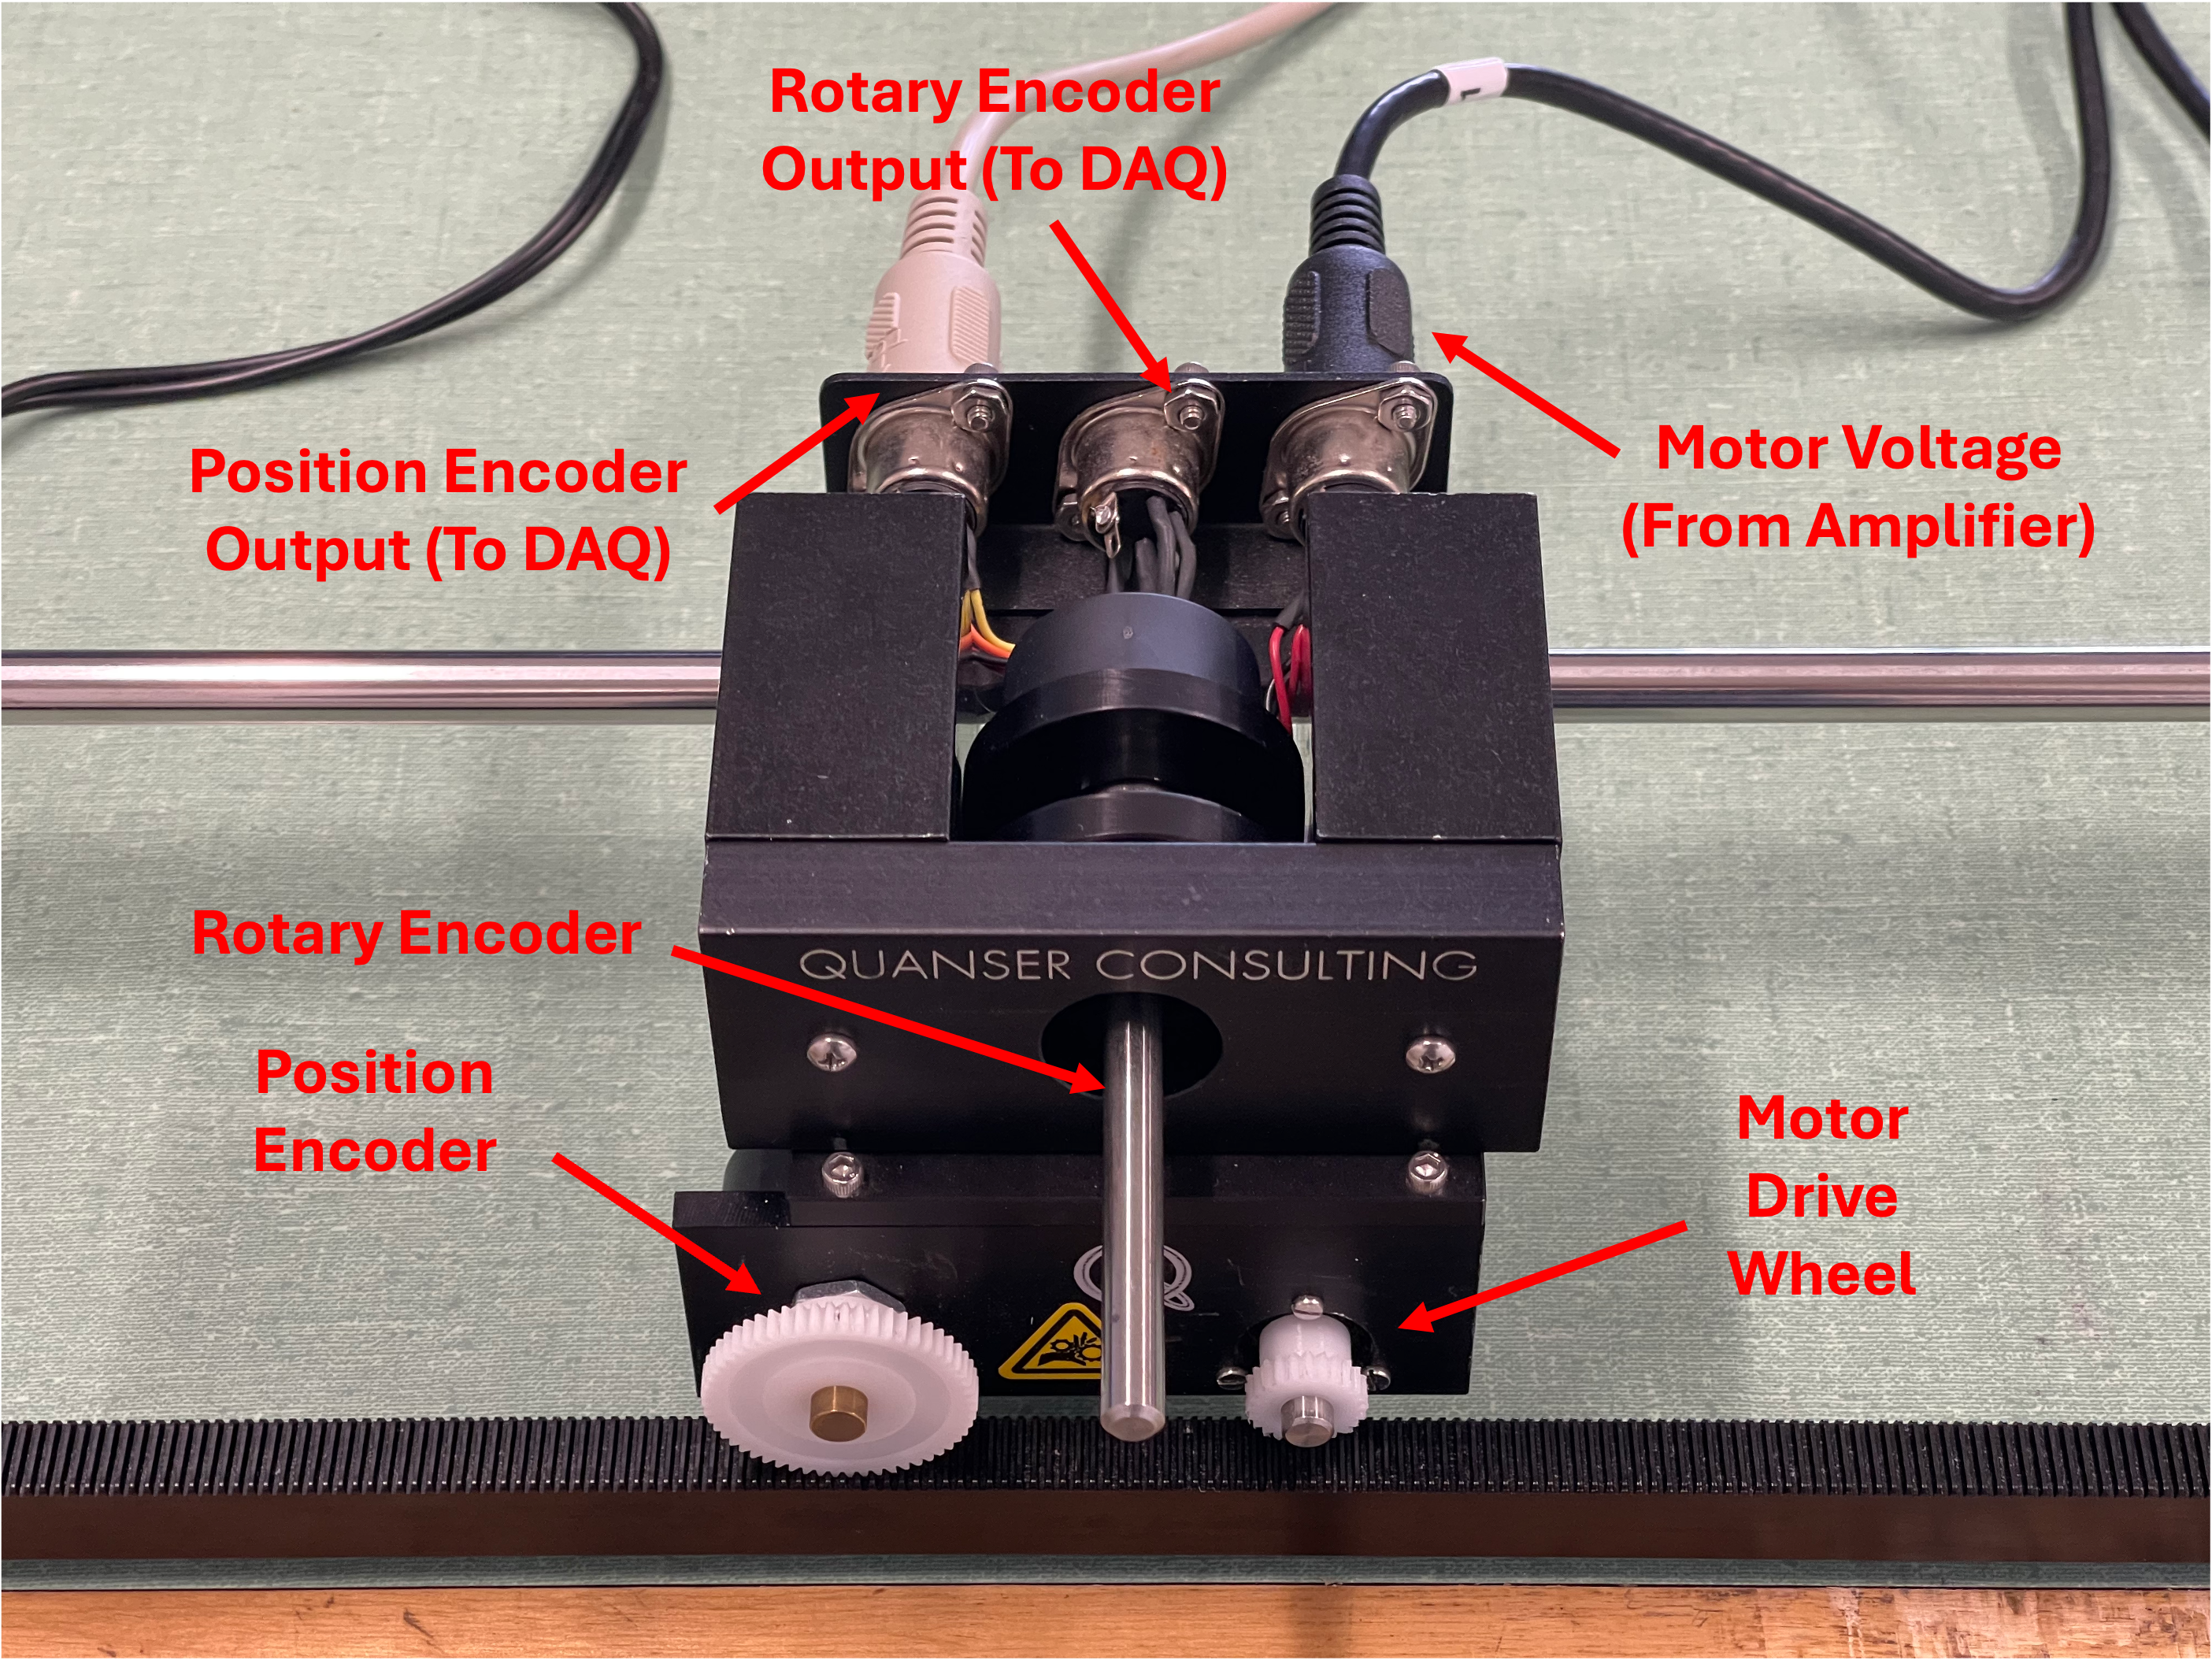
\includegraphics[width=.75\textwidth]{./Figures/cart_annotated.png}
  \caption{Quanser Linear Servo Base Unit (The `Cart')}
  \label{fig:cart}
\end{figure}






\section{General Info}
\begin{itemize}
  \item If the DAQ board light is off, check that the ribbon cables going to/from the PC are connected properly. If there is still an issue then the (minimum 1 Amp) fuse above the LED may need replacing. Make everything is completely unplugged from the DAQ board before doing this. Spare fuses can be found in a toolbox in the gray cabinet at the back right of the lab.
  \item If the DAQ board is not connecting to the PC and the light is on try restarting the computer.
  \item Contact the IT people for computer problems, MATLAB issues, and getting TA/student login access:
  \[\href{mailto:support@ece.ucsb.edu}{\texttt{support@ece.ucsb.edu}}\]
  \item Contact the ECE shop people for issues with the lab hardware:
  \[\href{mailto:shop@ece.ucsb.edu}{\texttt{shop@ece.ucsb.edu}}\]
\end{itemize}



\newpage
\section{Setup Instructions (ECE147A Lab 2)}
\subsection{Hardware}\label{subsec:hardware}
The \textit{MultiQ-4 Terminal Board} (Figure \ref{fig:q4_DAQ}) is a general purpose data acquisition and control board which has eight single ended analog inputs, eight analog outputs, sixteen bits of digital input, sixteen bits of digital output, three programmable timers, and eight encoder inputs decoded in quadrature. For the purposes of this lab, we will be primarily concerned with the analog outputs, the encoder inputs, and, to a lesser extent, the analog inputs.
\begin{figure}[H]
  \centering 
  \includegraphics[width=1\textwidth]{Figures/q4_daq.png}
  \caption{MultiQ-4 Terminal Board Schematic}
  \label{fig:q4_DAQ}
\end{figure}
\noindent Both the analog inputs and outputs are accessed via clearly labeled RCA jacks on the MultiQ-4 board and have a range of ±5 volts. The encoder inputs are accessed via a 5 pin DIN socket and connect directly to the experimental equipment.

\newpage
\subsubsection{Hardware Setup}\label{subsubsec:hardware_setup}
As a basic example, we will set up the system to read in the encoder from the motor cart and output a constant voltage to the motor.
\begin{enumerate}
  \item You must use \textbf{MATLAB R2023a} \textit{only}. The other versions will not work. Start SIMULINK and create a new model.
  
  %\item In the blank model window, choose \textbf{Simulation $\baro$ Mode $\baro$ External}
  
  \item Choose \textbf{Modeling $\baro$ Model Settings}
  
  \item Set the following parameters
  \begin{enumerate}
    \item Select \textbf{Solver} from the tree at the left
    \item Stop time: \textbf{inf} - or whatever $T_f$ is desired (in seconds)
    \item Solver options, solver type: \textbf{Fixed-Step}
    \item Solver options, solver: \textbf{discrete} if there are no continuous states. Select a solver like \textbf{ode4} if you are using continuous states (like a continuous transfer function)
    \item Solver options, Fixed-step size (under Solver details): \textbf{0.001}
    \item The settings are illustrated:
    \begin{figure}[H]
      \centering 
      \includegraphics[width=.9\textwidth]{Figures/fig2_solver.png}
      \caption{Configuration Parameters}
      \label{fig:4f_settings}
    \end{figure}
    \item Choose \textbf{Code Generation} in the tree on the left.
    \item Ensure the System target file is \textbf{quarc\_win64.tlc}. If not, select the \textbf{Browse} button and select it. The settings should look as follows. 
    \begin{figure}[H]
      \centering 
      \includegraphics[width=.9\textwidth]{Figures/fig3_codegen.png}
      \caption{RTW Parameters}
      \label{fig:4h_settings}
    \end{figure}
  \end{enumerate}
  \item Select OK and return to the SIMULINK model.
  \item In the SIMULINK Library Browser, find the \textbf{HIL Initialize} block. It is located in \textbf{QuaRC Targets $\baro$ Data Acquisition $\baro$ Generic $\baro$ Configuration}. You can also search by double clicking the model background. Add the block into your model.
  \begin{enumerate}
    \item \textit{Aside}: HIL stands for \textit{Hardware In the Loop}. It is a design technique in which the controller hardware is tested with a simulated plant. A flight simulator is an example; the pilot (controller) is connected to simulated inputs and outputs. The technique we are using in the lab is often called \textit{Rapid Control Prototyping}, where a PC controller is connected to actual plant hardware. If you are simulating everything on a computer, like in the prelab, you are doing \textit{offline simulation}.
  \end{enumerate}
  \item Double click on the \textbf{HIL Initialize} block in your model. Change the Board type to \textbf{q4}. Make sure the Board Identifier is \textbf{0}. Click Apply and Ok out of the block.
  \begin{figure}[H]
    \centering 
    \includegraphics[width=.75\textwidth]{Figures/fig4_HILinit.png}
    \caption{HIL Initialize Parameters}
    \label{fig:HIL_init_params}
  \end{figure}
  \item Add a \textbf{HIL Write Analog} block and a \textbf{HIL Read Encoder} block to your model. They are in \textbf{QuaRC $\baro$ Data Acquisition $\baro$ Generic $\baro$ Immediate I/O}.
  \item Connect these blocks as depicted in Figure \ref{fig:simple_model}. In this example, we place a simple constant output and a display for the encoder. \textit{For the purposes of this example, do not output more than 1 volt to the cart to prevent uncontrolled motion.}
  \begin{figure}[H]
    \centering 
    \includegraphics[width=.8\textwidth]{Figures/fig5_simplemodel.png}
    \caption{Simple Model}
    \label{fig:simple_model}
  \end{figure}
  \item When your model is ready, save it. From the \textbf{QuaRC} menu, select \textbf{Build}. MATLAB will compile your SIMULINK model into native machine code. You can check the status of the build by clicking \textbf{View diagnostics} at the bottom of the SIMULINK window. \textit{Every time you structurally change your model (add new blocks, rewire existing blocks) you will need to rebuild it or an error will occur.} 
  \begin{enumerate}
    \item \textit{Tip}: You do not need to rebuild the model if you are changing constants, or blocks that take a constant, like the gain of the gain block. You can even change these constants while the model is running and the change will take effect immediately. 
    \item \textit{Tip}: You can change the constants in a transfer function while stopped or running such that they do not affect the dimensions of the state. That is, the number of poles and zeros must remain the same. Any other change requires a rebuild.
    \item \textit{Use care when changing a running model! Be careful not to leave the model running by accident.}
  \end{enumerate}
  \item Ask your TA to set up the cart for motion. It should be placed in the center of the track and the Quanser Amplifier switched off.
  \item When the build is completed, go back to the model and choose \textbf{QuaRC $\baro$ Monitor \& Tune}. This downloads the compiled model to the QuaRC execution program and then model will run. The \textbf{Stop} button in the Quarc menu will stop the model as normal.
  \begin{enumerate}
    %\item \textit{Tip}: You can also click Connect to Target, followed by the SIMULINK Play Button. This is the same as using the QuaRC menu.
    \item \textit{Troubleshooting Tip}: If the SIMULINK time is not running (at the bottom of the model window), the QuaRC execution environment may have crashed. Try logging out and logging back in or rebooting the computer.
    \item \textit{Tip}: Suppose your model is running and MATLAB crashes. The model will continue to run. First, ensure the hardware is not damaged by lifting it off the track and then switching off the Amplifier.
    
    % After the hardware is safe, stop the model by checking for the Q icon in the system tray (by the clock in the lower right). If the Q icon is not there, start it from Start Menu $\rightarrow$ All Programs $\rightarrow$ Quanser QuaRC $\rightarrow$ Monitor. Right click the Q and choose \textbf{Stop all}.
  \end{enumerate}
  \item As the model runs, observe that moving the cart will change the encoder output, as shown on the display. Lift the cart up from the track and turn on the Quanser Amplifier. Observe the motor motion.
  \item Save your basic model to your network drive to use as a starting point for future designs.
\end{enumerate}



\subsubsection{Data Logging}\label{subsubsec:data_logging}
In the Real Time Windows Target, data is logged by scope blocks. Like an oscilloscope, to start the data logging procedure, a trigger is needed to initiate the process. A simple approach is to define a dedicated scope block, with one trigger signal entering it. Put a step function with a step time of 0.001 seconds, which corresponds to one sample time. This set-up will save all but the very first data point. To record data, follow the procedure below.
\begin{enumerate}
  \item Place a STEP function block from the SOURCES library and a SCOPE block from the SINKS library in your model.
  
  \item Name the SCOPE block TRIGGER SCOPE so that it is easy to identify in a list.
  
  \item Set the step time of the STEP block to the time you wish to begin saving data. Set the Initial Value and Final Value to 0 and 1 respectively.
  \begin{figure}[H]
    \centering 
    \includegraphics[width=.7\textwidth]{Figures/fig6_stepfunc.png}
    \caption{Step Function Block as a Trigger Signal}
    \label{fig:step_trigger}
  \end{figure}
  \item Go to the HARDWARE menu and select CONTROL PANEL.
  
  \begin{figure}[H]
    \centering 
    \includegraphics[width=.65\textwidth]{Figures/fig7_ecmpanel.png}
    \caption{Hardware Control Panel}
    \label{fig:emc_panel}
  \end{figure}
  \item Click on the SIGNALS AND TRIGGERING button.
  
  \item Select the TRIGGER SCOPE block from the list and click on the TRIGGER SIGNAL button. This selects the input to the scope block as the trigger signal. 
  
  \item In the TRIGGER area make sure that SOURCE = SIGNAL, MODE = NORMAL, DELAY = 0, and set DURATION = $T_f/T_s$. The duration is the number of samples allotted in memory for each signal being logged. If we have a simulation time of $T_f$ = 10 seconds and our sampling time $T_s$ = 0.001, then 10/0.001 = 10,000 samples. If you actually run the model longer than $T_f$, then the data in memory will be overwritten when Tf/Ts samples have passed. Check Figure \ref{fig:trigger_config}.
  
  \item In the TRIGGER SIGNAL area make sure that DIRECTION = EITHER or RISING, and LEVEL = 0.5. Our STEP signal will transition from 0 to 1 at 0.001 seconds, and is a rising edge. When it crosses the value 0.5 this will initiate the signal logging.
  \begin{figure}[H]
    \centering 
    \includegraphics[width=.8\textwidth]{Figures/fig8_signals_and_triggering.png}
    \caption{Configuring the Trigger Signal}
    \label{fig:trigger_config}
  \end{figure}
  \item Open all SCOPE blocks and configure them in the following way. 
  
  \item Click the SCOPE PROPERTIES Icon (gear icon), and select the LOGGING tab. 
  
  \item Make sure Limit data points to last is UNCHECKED.
  
  \item If you wish to save the data gathered by the scope, CHECK the Log data to workspace box, and give the Variable name a unique and meaningful name for easy reference later. In the SAVE FORMAT menu choose the ARRAY option. Click Apply and Ok out of the menu.
  
  \item \textit{Hint}: Once you have set these parameters as you like, you can RIGHT CLICK on a scope block, drag and drop, and a copy of that block will be placed where you let go of the mouse. The new block will have all of the parameters of the previous, except the Variable name, that will be different and should be changed to something meaningful. 
\end{enumerate}


\section{Demo Model}
\begin{enumerate}
  \item Generate the SIMULINK diagram shown in Figure \ref{fig:simulink_loopback}. The Sine wave should have a relatively low magnitude of around 0.75 and a frequency of around 1 Hz.
  \begin{figure}[H]
    \centering 
    \includegraphics[width=.75\textwidth]{Figures/fig10_loopback.png}
    \caption{SIMULINK Loopback System}
    \label{fig:simulink_loopback}
  \end{figure} 
  \item The output is an integer corresponding to counts. There is certain number of counts/revolution of the optical encoder's shaft. The gain seen in the figure is the `conversion factor for encoder reading'. It should be $1/35000$, ask your TA to make sure. The $1/35000$ factor means that when encoder counts 35,000 in one direction it has moved 1 meter. 
  \item After creating the system diagram and saving it, build the model following steps written in Section \ref{subsubsec:hardware_setup}. This generates the real-time code for the diagram. Wait until the compilation is complete. The SIMULINK window diagnostics panel displays the progress of the code generation task and, when it is complete, the following message appears:
  \begin{figure}[H]
    \centering 
    \includegraphics[width=.6\textwidth]{Figures/codegen_message.png}
    \caption{Successful Code Generation Message}
    \label{fig:build_success}
  \end{figure}
  \item Check the necessary wires:
    \begin{enumerate}
      \item Connect Analog Output 0 of the MultiQ-4 board to the Quanser Amplifier “Amplifier Command" via the red RCA cable.
      \item Connect the Quanser Amplifier “To Load" (6 pin DIN) to the motor cart's motor (4 pin DIN). 
      \item Connect the optical encoder which measures cart position (5 pin DIN) to MultiQ-4 Encoder Input 0 (5 pin DIN). 
    \end{enumerate}
  \item Make sure the Amplifier Gain is set to 1x. Ask for the TA’s permission to turn the Quanser Amplifier on. In unexpected situations, turn it off. Place the motor cart in the center of the track.
  \item You should be able to run the model by clicking MONITOR \& TUNE. Do not move the cursor. Press STOP immediately if needed.
\end{enumerate}


\end{document}